%########
% Hvad er totality?
% Hvorfor totality?
% Totalitet skal bevises
%% Hvordan beviser man det?
% Hvorfor er totalitet ikke standard?
% Partiality
% Coverage
% Termination
% Produktivitet

% Finite prefix af coinduktiv data ved endeligt antal unfolds
% Partielle funktioner defineres ved subset-intuition

% Ny viden: Hvorfor totality?, Hvad består totalitet af? Produktivitet vs. terminering, total vs. partiel funktion
%########

\section{Totality and Total Functional Programming}
\label{sec:totality}
Totality is a property of functions. In the context of functional programming,
totality is thus a property of programs, assuming that our programming language
models mathematical functions. 

\begin{definition}[\textit{Total function}]
\label{def:total_function}
A function $f$ with domain $A$ and codomain $B$ is total if for \emph{every}
element $x\in A$, $f$ assigns a value
$f x\in B$\,\citep{Turner04totalfunctional}.
\end{definition}

Within Definition \ref{def:total_function} is the implicit assumption that each
such assignment happens in finite time; if $f$ requires infinite time to compute
$f y$ for some input $y\in A$, then $f$ does not assign a value $f y\in B$, and is
therefore \emph{undefined} for $y$. In this case, $f$ is not total. Programming
solely with total functions has attracted more and more attention in recent
years, and has even given rise to the aptly named discipline of ``total
functional programming''. But why should we care whether the programs we write
are total?

\subsection{Partiality and Partial Functional Programming}
An appreciation of totality is perhaps best achieved by understanding its
counterpart, \emph{partiality}. Like totality, partiality is also a property of
functions. 

\begin{definition}[\textit{Partial function}]
  A function $f$ with domain $A$ and codomain $B$ is partial if $f$ is undefined
  for some $x\in A$. Specifically, if $f$ is a partial function, then there
  exists a total function $g$ with domain $A'$ and codomain $B$, such that
  $A' \subset A$.
  % inhabitant $x\in A$, $g$ does not assign a value $g x\in B$. More precisely, there exists
  % an element $x\in A$ for which $g$ is undefined, i.e. either $g$
  % requires infinite time to compute $g x$, or the definition of $g$ has no
  % reduction rule for $x$.
  \centering
  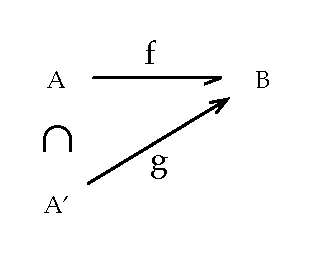
\includegraphics[scale=0.8]{figures/partialfunc}
\end{definition}

For input  where a partial function is undefined, we say that
the function evaluates to $\bot$, here denoting either an exceptional state (a
run-time error) or infinite recursion\,\citep{Turner04totalfunctional}. The
implications of programming with partial functions (``partial functional
programming'') is greater than it may seem: Whenever we have no guarantee that a
function is total, $\bot$ is a possible result, which should be handled
properly. When $\bot$ signifies that program evaluation has reached an
exceptional state, an error or exception handling machinery can be set in motion
to recover from the situation, if possible. But when program evaluation reaches
an infinite recursion, meaningful recovery becomes impossible. First, due to the
undecidability of the halting problem, it is impossible to determine whether an
infinite recursion has, in fact, been reached. Secondly, it might not be
possible for the runtime system to simply stop evaluating the infinitely
recursive function and move on, since later computations could depend on the lost
output value. With this in mind, handling $\bot$ cases for all partial functions
is clearly undesirable, and simply doing nothing is not necessarily a sensible
solution. The main selling point of total functional programming is therefore
that $\bot$ is never a possible result of program evaluation.

\subsection{A Total Program is a Proof}
Another advantage of programming with total functions is that our programs can
act as proofs. The Curry-Howard isomorphism identifies a deep connection
between logic and computer
programs\,\citep{Curry1934,Howard80,Wadler2014}. Within this connection, types
are identified as propositions, (total) programs as proofs, and evaluation of
programs as simplification of proofs. Consequently, a program can be viewed as a
proof script in a logic (which, in this case, is our programming language),
showing that a given proposition, specified by the program's type, holds. This
is not merely an academic curiosity, but leads to a situation where a program
can be \emph{correct by construction}\,\citep{Pierce:2002:TPL:509043} if its
type sufficiently describes the program's behaviour. The correctness of the
program can then be established statically by the type checker.

A partial function can never be correct by construction, since evaluating it
might lead to infinite recursion. Infinite recursion is logically equivalent to
Russell's paradox (the equivalent type theoretic formulation is given by
Girard's paradox\,\citep{Girard1972}), which is known to introduce an inconsistency into an
intuitionistic logic, and therefore also into the logic that is our programming
language. Any proposition can be deduced in an inconsistent logic, and as a
consequence, a partial function can never act as a valid proof.

%  which is the general notion that
% programs are proofs and types are propositions, a well-typed program $p$ of type
% $T$ constitutes a constructive proof of the proposition $T$. The proof is
% constructed by providing an inhabitant of the output type. If a total program $p$ has a domain $A$
% and a codomain $B$, and there is an $x\in A$, $p$ can construct a proof of $B$ by
% providing an inbitant of $B$ for $p x$. The implication of
% having programs as proofs is that given a type specification which is sufficiently
% strong, we can implement programs which are \emph{correct by construction},
% i.e. statically proven correct by the compiler. Partial functions cannot act as
% proofs, since $\bot$ is a possible result. If the aforementioned $p$ is a
% partial program, no inhabitant for $B$ can be provided for input where $p$ is
% undefined. 

\subsection{Ensuring Totality}
If have no guarantee that a function is total, then it must be assumed to be partial. To
obtain such a guarantee for an arbitrary function $f$, we must be able to
construct a proof showing that $f$ is total. A totality proof is twofold,
consisting of a proof of coverage and a proof that all invocations result in an
output value in finite time.

\begin{definition}[\textit{Covering function}]
  \label{def:covering_function}
  A function $f$ with domain $A$ and codomain $B$ is covering if its definition
  has a reduction rule for every inhabitant $x\in A$.
\end{definition}

Depending on whether the codomain of a covering function $f$ is an inductive or
a coinductive type, $f$ must be shown to be either \emph{terminating} or
\emph{productive} in order to ensure that all invocations of $f$ lead to a
result in finite time.

\begin{definition}[\textit{Terminating function}]
\label{def:terminating_function}
  A function $f$ with domain $A$ and codomain $B$, where $B$ is an inductive
  type, is terminating if for every inhabitant $x\in A$, the output value
  $f x\in B$ is \emph{fully} constructed in finite time.
\end{definition}

Since any inductive data has finite size by definition, a terminating function
terminates in the literal sense of the word: When the output has been
constructed, no further computations can be done for the given
input. Termination proofs are often constructed by showing that all recursive
invocations of a function happen on structurally smaller input. For
productive functions, this is may not the case.

\begin{definition}[\textit{Productive function}]
\label{def:productive_function}
  A function $f$ with domain $A$ and codomain $B$, where $B$ is a coinductive
  type, is productive if for every inhabitant $x\in A$, a finite number of
  unfoldings of the output value $f x\in B$ can be constructed in finite time.
\end{definition}

Because coinductive data is possibly infinite, a productive function continually
unfolds its output, providing each unfolding in finite time. Notably, it might
never terminate, since constructing an infinite term (e.g. a list of all prime
numbers) never comes to a natural end. Productive functions are therefore often
evaluated using a call-by-name strategy, computing exactly the number of
unfoldings needed, deferring the computation of the remaining term.  A proof
of productivity can be constructed by showing that the function definition in
question exhibits some continuity property, e.g. causality: that any output only
depends on previously computed values.

\subsection{Automated Totality Proofs}
Manually writing proofs of totality is clearly not feasible in practice, as it
must be done for every function in a program individually. Consequently,
automated construction of coverage, termination, and productivity proofs has
received much attention in the community in recent years, a development which
will be outlined in Chapter~\ref{cha:related-work}. Most techniques are either
based on a purely syntactical analysis of terms or on type checking, where the
type of a program is decorated with auxiliary information. A popular and purely
syntactical technique for automating termination proofs is to analyze whether a
program is size-change terminating\,\citep{LeeJones01SizeChange} by tracing
(mutually) recursive calls in a statically constructed call graph. Syntactic
guardedness, which will be the subject of Section~\ref{sec:synt-guard-1}, is a
purely syntactical method for approximating productivity, whereas guarded
recursion, covered in Section~\ref{sec:guarded-recursion}, is a type-based
approach to constructing productivity proofs. A full automation of guarded recursion
proofs has yet to be described.

% Equational reasoning?
% partiality and partial functions
% recursive and corecursive functions
% Turing-completeness and corecursion
% Curry-Howard

%%% Local Variables:
%%% mode: latex
%%% TeX-master: "../../copatterns-thesis"
%%% End:
